记录上一个访问的边时要记录边的编号,不能记录上一个过来的节点(因为会有重边)!!!

(如果选择在加边的时候特判,注意编号问题:用输入顺序来对应数组中位置的时候,重边跳过,但是需要 tot+=2。)

圆方树示意图:

\begin{figure}[H]
    \centering
    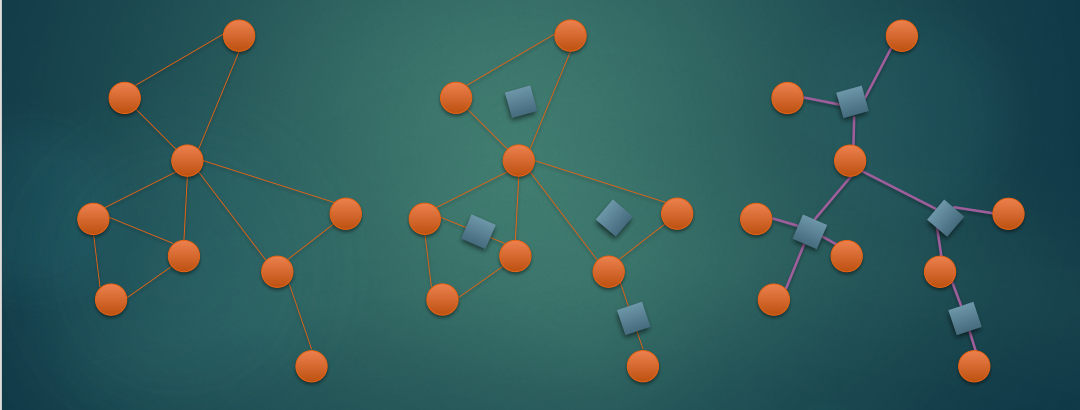
\includegraphics[width=0.45\textwidth]{src/graph/tarjan-tree.png}
    \caption{圆方树示意图}
\end{figure}

\inputminted{cpp}{src/graph/tarjan.cpp}